\documentclass[tikz,border=5pt]{standalone}
\usepackage{fontspec}
\setmainfont{Times New Roman}
\usepackage{unicode-math}
\setmathfont{Cambria Math}
\usetikzlibrary{shapes.geometric,shapes.misc,positioning,fit,backgrounds,arrows.meta,calc}

\begin{document}
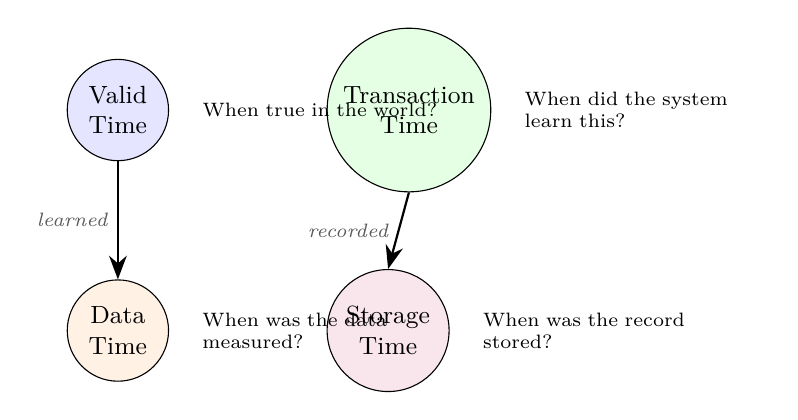
\begin{tikzpicture}[
    clock/.style={circle, draw, minimum size=1.2cm, align=center, font=\small},
    arrow/.style={-{Stealth[length=3mm]}, thick},
    label/.style={font=\scriptsize\itshape, text=gray!70!black},
]

% Four clocks arranged in a 2x2 grid
\node[clock, fill=blue!10] (vt) at (0,0) {Valid\\Time};
\node[clock, fill=green!10, right=2cm of vt] (tt) {Transaction\\Time};
\node[clock, fill=orange!10, below=1.5cm of vt] (dt) {Data\\Time};
\node[clock, fill=purple!10, right=2cm of dt] (st) {Storage\\Time};

% Annotations
\node[right=0.3cm of vt, font=\scriptsize, text width=3cm] {When true in the world?};
\node[right=0.3cm of tt, font=\scriptsize, text width=3cm] {When did the system learn this?};
\node[right=0.3cm of dt, font=\scriptsize, text width=3cm] {When was the data measured?};
\node[right=0.3cm of st, font=\scriptsize, text width=3cm] {When was the record stored?};

% Arrows showing temporal flow
\draw[arrow] (vt.south) -- node[left, label] {learned} (dt.north);
\draw[arrow] (tt.south) -- node[left, label] {recorded} (st.north);

\end{tikzpicture}
\end{document}
